\section{Vision and tension based inertial identification}
\label{sec:identification}
\subsection{Surface reconstruction and visual pose}
The initial object scan is acquired in a known static installation fixture. Depth measurements are projected into calibrated coordinates and fused from twelve views. Voxel reduction produces a surface point set with up to 6000 points. The known fixture fixes the initial scan frame, including the orientation of a geometrically symmetric cuboid. Subsequent registration operates on the acquired surface rather than on a supplied ideal object mesh.

During transport, two virtual RGB-D views provide partial surface observations. A predicted search region follows the most recent registered pose, and geometric correspondence rejects points inconsistent with the reference surface. Point-cloud alignment follows the iterative registration principle~\cite{icp1992}; temporal prediction initializes each local alignment. For the forked object, chromaticity statistics learned during the fixture scan filter background points while preserving thin prongs and cavity boundaries. The initial scan precedes rope installation, while transport images include the rigging. No fiducial marker or renderer object-ID mask is used.

The resulting visual observations are timestamped by exposure time. Tensions and aircraft endpoint telemetry are sampled at the same time. Their association is retained when image processing finishes later. The estimator therefore uses cable directions and load pose from a common physical instant rather than combining delayed geometry with current tensions. Nine consecutive observations are fitted by a local cubic polynomial, with derivatives assigned to the center observation. At the 10 Hz request rate this introduces an approximately 0.4 s fixed lag. Only observations already received enter an identification solve. This 0.4 s derivative lag applies to preparation-phase parameter estimation. During transport, the controller uses the most recent visual pose and a velocity-based prediction to the current control time; its reported sensor age is the exposure-to-control age, without the preparation derivative lag.

\subsection{Integral momentum observations}
An integral formulation avoids differentiating the visual trajectory twice. About a fixed world origin, payload linear and angular momenta are
\begin{align}
 P&=mv+\omega\times Rh,\\
 H&=p\times P+(Rh)\times v+RJ_OR^T\omega.
 \label{eq:momentum}
\end{align}
Both are linear in $\theta$, so define $[P^T,H^T]^T=Y_M\theta$. Gravity contributes the parameter-linear wrench
\begin{equation}
 w_g=\begin{bmatrix}mg\\(mp+Rh)\times g\end{bmatrix}=Y_g\theta.
\end{equation}
The measured cable wrench about the same origin is
\begin{equation}
 w_c=\begin{bmatrix}\sum_i T_iq_i\\\sum_i a_i\times(T_iq_i)\end{bmatrix}.
\end{equation}
For every complete interval $[t_a,t_b]$, integration gives
\begin{equation}
 \left(Y_M(t_b)-Y_M(t_a)-\int_{t_a}^{t_b}Y_g\,dt\right)\theta
       =\int_{t_a}^{t_b}w_c\,dt.
 \label{eq:integral}
\end{equation}
The implementation uses trapezoidal integration over nonoverlapping 0.4 s intervals. Stacking the resulting equations produces $A\theta=b$. A translated fixed world origin near the first observation reduces unnecessary moment lever arms while preserving Eq.~\eqref{eq:integral}.

\subsection{Shape-supported moment fitting}
Let $s_r$ be candidate mass-support locations inside the convex hull of the reconstructed surface. A nonnegative mass $\mu_r$ at each location contributes to mass, first moments and inertia. With a small isotropic cell-inertia term $\epsilon I$, the contributions are
\begin{equation}
 m=\sum_r\mu_r,\quad h=\sum_r\mu_rs_r,\quad
 J_O=\sum_r\mu_r\big(\norm{s_r}^{2}I-s_rs_r^T+\epsilon I\big).
 \label{eq:support}
\end{equation}
Write these relations compactly as $\theta=B\mu$. The estimate is obtained from
\begin{equation}
 \begin{split}
 \min_{\mu}\;&\tfrac12\norm{AB\mu-b}^{2}+\tfrac{\lambda}{2}\norm{\mu}^{2}\\
 \text{s.t. }&\mu\geq0,\qquad m_{\min}\leq\mathbf{1}^{T}\mu\leq m_{\max}.
 \end{split}
 \label{eq:fit}
\end{equation}
This is a convex quadratic conic program~\cite{boyd2004}. The nominal fit minimizes the unwhitened residual in SI units. Linear- and angular-impulse residuals are reported separately. To assess the relative scaling of their different units, the supplementary analysis rescales moment rows by $1/L$ for $L\in\{0.25,0.5,1,2\}$ m and refits the same observations; this is a unit-weighting sensitivity test, not covariance whitening. The support spacing is 0.08 m, $\epsilon=5\times10^{-5}$ m$^2$, $\lambda=10^{-8}$, and the prescribed mass interval is 0.7--1.5 kg. A limited set of hull vertices supplements the interior grid. Nonnegative support guarantees moments realizable by mass within the scanned convex envelope, following the mass-distribution interpretation of inertial parameters~\cite{wensing2018}.

For a nonconvex object, this hull is a conservative envelope of possible mass locations. It serves the moment estimation problem, whereas the reconstructed nonconvex surface serves collision evaluation. The envelope therefore imposes moment consistency and a spatial outer bound, rather than identifying a material-only density. The weights in Eq.~\eqref{eq:fit} are one representation of the fitted moments: many different internal distributions can generate the same ten parameters. The estimated quantities passed to the planner are $\hat m$, $\hat c$ and $\hat J_O$.

An activation test checks the measurement geometry before using these moments. The normalized observation matrix must have rank ten, condition number at most 1000 and at least eight complete integral windows. The minimum eigenvalue of the mean $\omega\omega^T$ matrix must exceed $10^{-4}$ s$^{-2}$. Measured tension must exceed its 0.01 N error bound, and the central second-moment matrix $\frac12\operatorname{tr}(J_C)I-J_C$ must be positive definite. These conditions connect activation to angular excitation, valid tension measurements and physical moment consistency.

\begin{figure*}[t]
\centering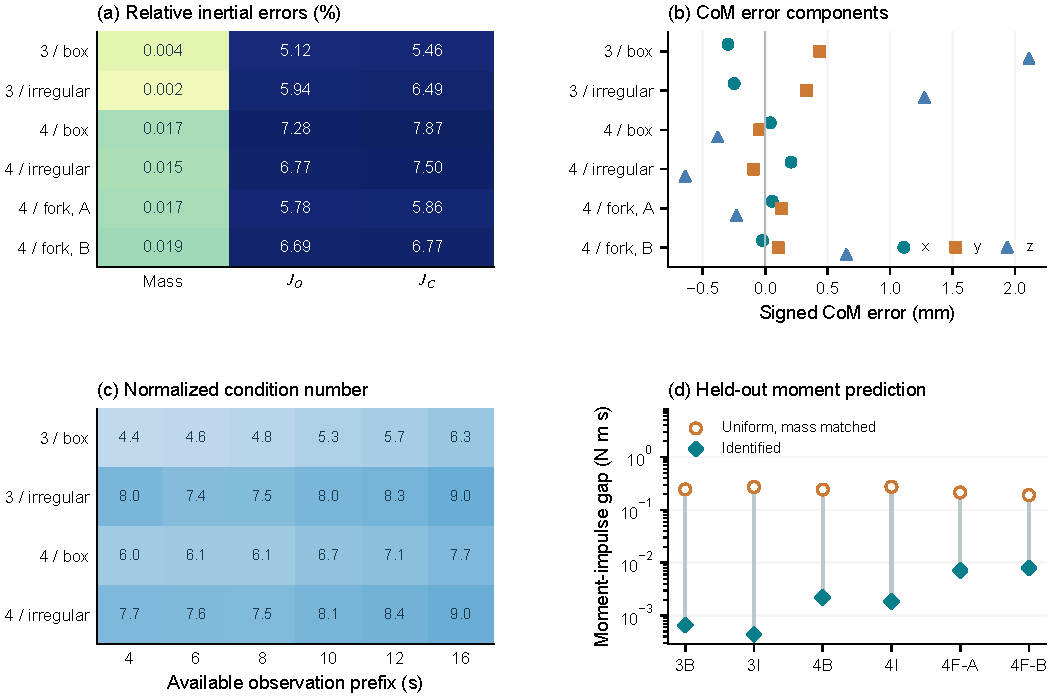
\includegraphics[width=\textwidth]{fig03_identification.pdf}
\caption{Inertial accuracy and predictive evaluation. (a) Relative mass and inertia errors in six recorded executions; inertia errors use the Frobenius norm. (b) Signed CoM errors in the scan frame; circles, squares and triangles denote the $x$, $y$ and $z$ components. (c) Condition number of the column-normalized integral observation matrix using only data available by each prefix; all displayed systems have rank ten. (d) RMS difference from the true-inertia moment-impulse prediction on transport observations excluded from fitting, comparing identified and mass-matched uniform models. Fork A and B denote the moderate- and large-rotation courses. Heatmap colors use logarithmic scales; cell annotations give the numerical values.}
\label{fig:identification}
\end{figure*}
